We now adopt a goal-based approach to determine the requirements associated with each one of the goals we have elaborated in Chapter 1.\\
We'll start numbering and exploring the goals we submitted.

\begin{itemize}

            \item \textit{[G1]} System allows guest user to register with an username ad and a password; to complete the procedure user should confirm by 
               
                  \begin{itemize}
                        \item [R.1.1] System lets registering user choose an username and password
                        \item [R.1.2] Every username corresponds to a single user
                        \item [R.1.3] Duplicate usernames aren’t allowed
                        \item [R.1.4] Registering user can't be already registered
                        \item [R.1.5] An unregistered user is locked out the application and can only see registration page
                        \item [R.1.6] User has to confirm by mail his registration
                        \item [R.1.7] User can save its credit card data and link the to its account
                        \item [R.1.8] New user registration is successful only after data is stored on Travlendar+ server and a confirmation is received by the system
                        \item [R.1.9] User can link season passes to his account
                        \item [R.1.10] Each modification made to a user account must be saved into Travlendar+ Server to be made effective
                  \end{itemize}
             
\item \textit{[G2]} System Login

                  \begin{itemize}
                        \item [R.2.1] User must be already registered to perform correct login
                        \item [R.2.2] User must remember username and password to login
                        \item [R.2.3] Only a correct combination of username and password will grant access
                        \item [R.2.4] Application will implement a password retrieval mechanism
                  \end{itemize}
                  
                  
\item \textit{[G3]} The application integrates a calendar and a timetable

                  \begin{itemize}
                  
                  \item [R.3.1] The calendar and the timetable must be two different views 
                  \item [R.3.2] Calendar must encompass month by month views
                  \item [R.3.3] Timetable must encompass day by day views, reserving hourly slots to events
                  \item [R.3.4] Calendar and Timetable views can be modified only by the user inserting events. No other way is allowed to modify the information they contain
                  \item [R.3.5] Calendar and Timetable for each user are remotely copied on Travlendar+ Server every time a user creates/modifies /deletes an event
                        
                  \end{itemize}
                  
\item \textit{[G4]} Registered User can create appointments 

 \begin{itemize}
                        \item [R.4.1] User has to be registered and logged in the system in order to create an
appointment
                        \item [R.4.2] Appointments can be divided into work appointments (or meetings) and personal appointments
                        \item [R.4.3] Appointments require a location, a starting time and an end time
                        \item [R.4.4] Appointments location must be within the boundaries of the operative zone
                        \item [R.4.5] There cannot be appointments with the same name, location and time
                        \item [R.4.6] System must check suitability of created new entries based on already existing appointments
                        \item [R.4.7] Appointment start time can't precede the actual system time at the moment of inserting it                                 														\item [R.4.8] User can select favourite travel means and priority for each appointment
                        \item [R.4.9] Each appointment must be associated to a level priority
                        \item [R.4.10] The creation of an appointment must be remotely saved on Travendlar+ server in order to be successful and completed
                        
                  \end{itemize}
                  
\item \textit{[G5]} Registered Users can edit appointments

                  \begin{itemize}
                       \item  [R.5.1] A modified meeting must respect all the constraints imposed during the creation of a new meeting, as the requirements in [G4]
                       \item [R.5.2] A meeting can be modified up until its end time
                       \item [R.5.3] If the location of the meeting is modified , the system behaves as if such an event was inserted for the first time, calculating all possibile conflicts with pre-existing event
                       \item [R.5.4] No limit actually exists on the amount of times an event can be modified within the aforementioned constraints 
                       \item [R.5.5] A modification must be correctly saved on the remote Travlendar+ server in order to be succesful and completed              
                       \item [R.5.6] Deleting an appointments belongs to the set of modifications

                 \end{itemize}

\item \textit{[G6]} The application can automatically compute a personalized selection of travel times between appointments to choose from

                  \begin{itemize}
                        \item [R.6.1] The application must refer to Travel Logic for the expected travel time 
                        \item [R.6.2] The application can suggest a combination of various means to reach the desired destination
                        \item [R.6.3] In case of mixed travel means, distances must be calculated splitting the distances and submitting them to Travel Logic. Same goes with public means stop and shared vehicles positions
                        \item [R.6.4] Starting location for travel can be inserted manually, retrieved by the previous event or calculated through geo-localization
                        \item [R.6.5] The application must rank the suggestions according to their priority, presence of prefered travel means, time required
                        \item [R.6.6] The registered user can choose to filter out specific travel means
                        \item [R.6.7] Favourite travel means associated to an appointment must always show up
                        \item [R.6.8] In case two or more appointments overlap, an appointment with higher priority is considered automatically chosen and all the remaining ones are arranged according to their priority. Warnings must follow as expected
                        \item [R.6.9] The route can include intermediate destinations before the final, target one 
                        \item [R.6.10] When a shared vehicle is suggested the parking zone nearest to the destination must be always inserted among the intermediate destinations 
                        \item [R.6.11] The sytem must grant to know daily scheduled times for public transportation through its APIs
                        \item [R.6.	12] When an event is only one hour away the system must notify the user with an updated list of travel time so he can choose
                        \item [R.6.13] According to real world data, each travel must have associated to itself the carbon footprints
                       	\item [R.6.14] Travels that do not satisfy all User's contraint must be excluded
                        
                        
                  \end{itemize}
                  
\item \textit{[G7]} User can choose a solution among the scheduled ones 

                   \begin{itemize}
                        \item [R.7.1] Selecting a solution that is not a personal vehicle must show both intermediate and final destinations
                        \item [R.7.2] The application must arrange a navigable view of feasible solutions
                        \item [R.7.3] Choosing a solution that includes a public transportation mean must show the user the possibility to buy a ticket 
                        \item [R.7.3] Choosing a solution that includes a shared vehicle must show the user the possibility to locate and rent such a vehicle
                        \item [R.7.4] Choosing a solution must not be definitive
                        \item [R.7.5] Since an hour from the start of an event every 15 minutes system must notify user in case a new and faster travel solution has appeared in his current location or if his travel mean has delays that shift its speed rank by comparison to other solutions
                        \item [R.7.6] System must recognize by itself through geolocalization that a user reached destination, or he can manually tell the program
                  \end{itemize}
                  
\item \textit{[G8]} The application warns the user if locations are unreachable in the allotted time

                   \begin{itemize}
                        \item[R.8.1] The application must realize if the alloted time is sufficient from either the last event, current location or manually inserted location
                        \item[R.8.2] The application must use as a reference the time to cover distance between the starting place and the destination one, using the futured scheduled time for public transportation if necessary
                   			\item [R.8.3] Warning must arrive also while on the road if the travel mean is no longer suitable, or the best solution, as detailed in [G7] Requirements
                   			\item [R.8.4] When user reaches destination warnings must stop automatically
                   			\item [R.8.5] Warnings can be disabled on the road by the user
                   \end{itemize}

\item \textit{[G9]} Allow users to put constraints on different travel means and limit carbon footprints

											\begin{itemize}
											
														\item[R.9.1] User must be able to rule out vehicles from system scheduler
														\item[R.9.2] When the option of limiting carbon footprints gets enabled the associated CO2 consumed by each travel must be taken into account in travels scheduling
														\item[R.9.3] User must be able to forbid travel means within time spans, also periodical ones
														\item[R.9.4] User must be able to put a constraint on the maximum amount of space and time he can give to each travel mean
														\item[R.9.5] User must be able to put a constraint on the number of transporation of travel means adopted for a single travel
														\item[R.9.6] User must allow at least a single travel mean 
														\item[R.9.7] If no travel can be displayed according to user preferences, the system must suggest to show results that has been filtered out														
																						
											\end{itemize}



\item \textit{[G10]} The application features additional user’s privileged time spans 

											\begin{enumerate}
														\item[R.10.1] Privileged time spans must filter out any travel solution they overlap 
														\item[R.10.2] Privileged time spans can be periodic
														\item[R.10.3] Privileged time spans can be customized depending on the day of the week and hour of the day
														\item[R.10.4] Even periodic privileged time spans must be customizable with respect to the particular day of the week and hour of the day, increasing or decreasing their length
														
											\end{enumerate}

\item \textit{[G11]} The application allows to buy tickets for public services

													\begin{enumerate}
														\item[R.11.1] Buying a ticket must reroute the user to the corresponding payment service
														\item[R.11.2] User must be able to choose among the different purchase options offered by the public transportation service provider
													\end{enumerate}

\item \textit{[G12]} The application allows the nearest shared vehicle to be found and reserved

                   \begin{itemize}
                        \item [R.12.1] A shared vehicle must necessarily belong to a bike-sharing service or a car-sharing service
                        \item [R.12.2] All services linked to shared vehicles must be automatically disabled if the location of a meeting out of the boundaries of the influence zone
                        \item [R.12.3] All sharing services have their own API and they must be referenced by our mobile application
                        \item [R.12.4] To find or reserve a vehicle it is required by our system the access to the external API of the required service
                        \item [R.12.5] To find or reserve a vehicle it's required that the user logins into the external corresponding service
                        \item [R.12.6] The external service can communicate with our mobile application. In case of reservation Travlendar+ checks if the mobile app corresponding to the desired services is installed on the system. All the following steps take place within such an environment, until control is returned to Travlendar+
                        \item [R.12.7] The location of all the vehicles are shown in the same view, merging data from different APIs
                        \item [R.12.8] When an user decides to rent a car it must be redirected to the corresponding vehicle sharing service, until he's ultimated the rental and gets redirected back to Travlendar+
                        \end{itemize}

\item \textit{[G13]} The application integrates a map system
                   
                  \begin{itemize}
                        \item [R.13.1] The map must be submitted by an external service (in our case we'll select Google APIs)
                        \item [R.13.2] User can navigate through the map indipendently from its current location
                        \item [R.13.3] User can search for a specific location
                        \item [R.13.4] The mobile device can track its current position through geo-localization
                        \item [R.13.5] Position of out the operative zone can't be accepted by the system and won't be displayed
                   \end{itemize}


            \end{itemize}



\vfill

\subsubsection{Use case diagram}
	A global picture of the system interaction with actors is provided here by means of use case diagrams. Following, an analysis of the most interesting use case situations derived from scenarios is presented.

	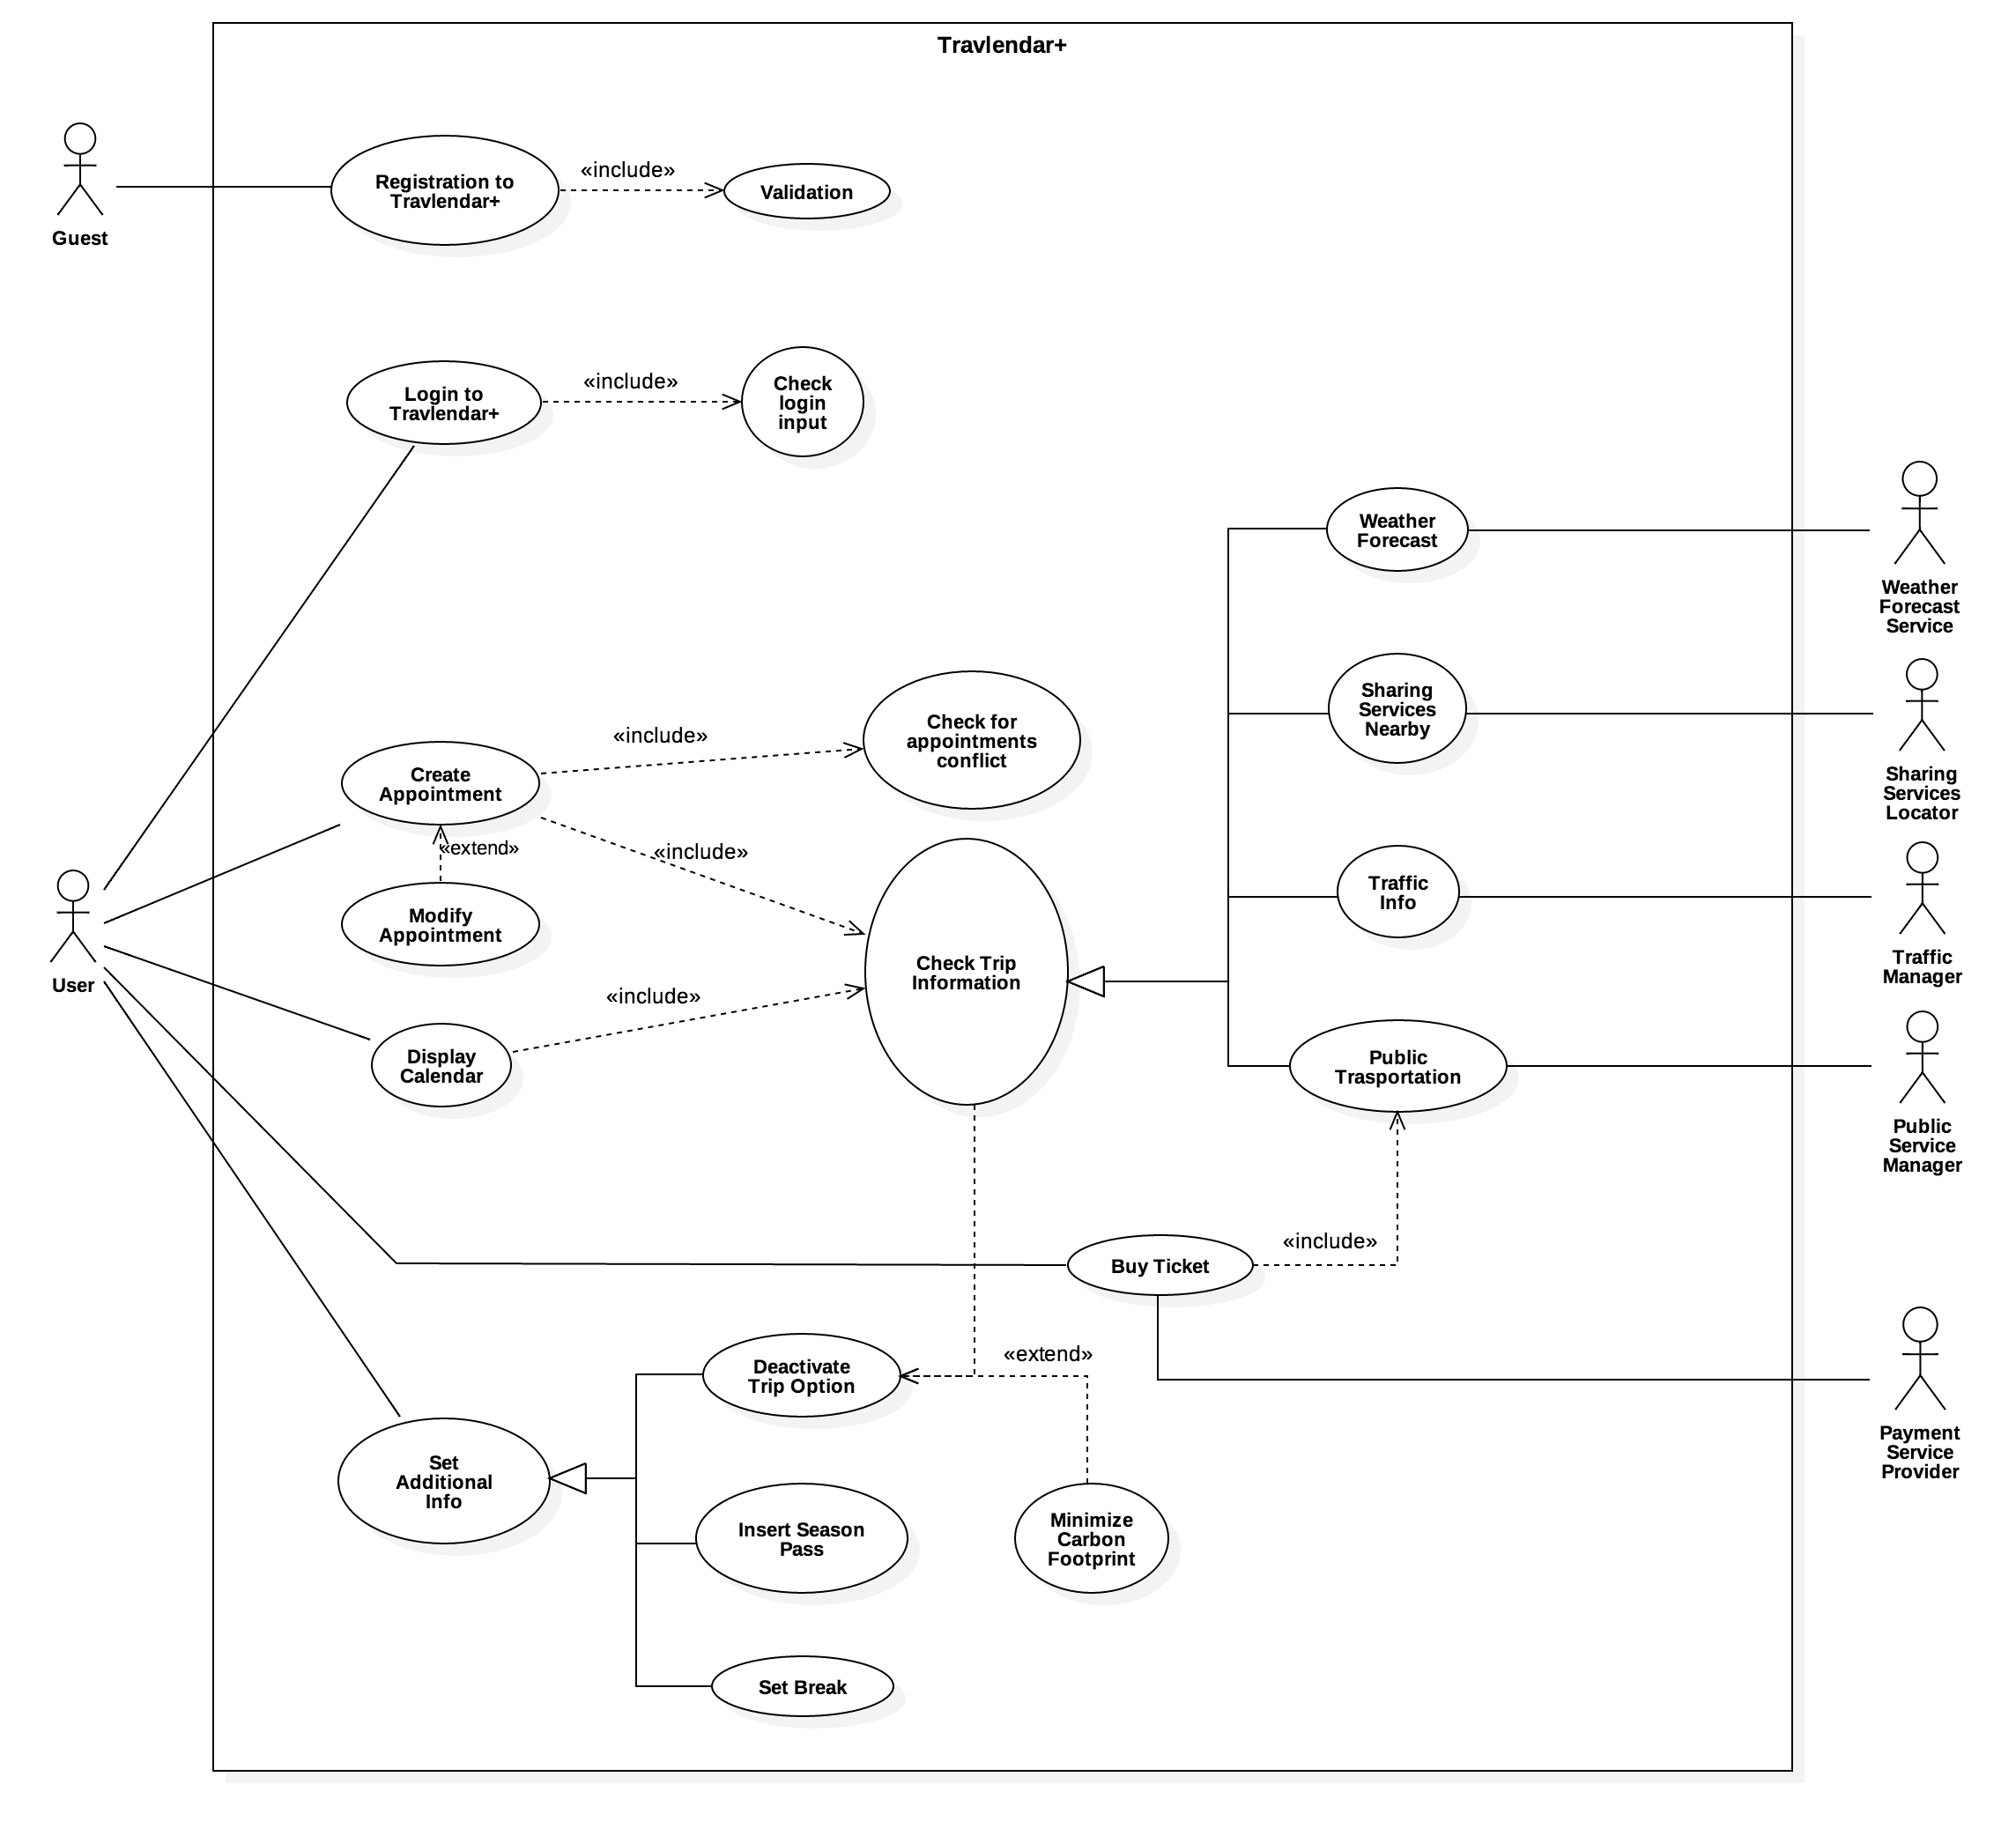
\includegraphics[width=\textwidth]{img/uml/useCase.png}
	
	\vfill
	
%%% CREATE A NEW EVENT %%%	
	\paragraph{Use Case 1: Create a New Event}
	
		\begin{tabular}{| l | p{0.8\textwidth} | }
			\hline
			\hline
			Actor	&		User. \\
			\hline
			Input Condition		&		User is already logged in into \textit{Travlendar+}. \\
			\hline
			Event Flow		&		\begin{enumerate}
												\item User click on "\textit{create event}".
												\item User set day, time, place, and event type.
												\item System checks if the new event overlap with already existing events or lunch period.
												\item	 System calculate, ranks and shows multiple solution depending on user travelling preferences.
												\item User select one solution as preferend one.
											\end{enumerate} \\
			\hline
			Output Condition		&		\textit{Tralvendar+} shows calendar main page with the new event. \\
			\hline		
			Exception		&		\begin{itemize}
											\item[-] Created event overlaps with already existing events.
											\item[-] There are no feasible solution.
										\end{itemize} \\
			\hline
			\hline
		\end{tabular}


%%% MODIFY EVENT %%%

	\paragraph{Use Case 2: Modify Event}
	
		\begin{tabular}{| l | p{0.8\textwidth} | }
			\hline
			\hline
			Actor	&		User. \\
			\hline
			Input Condition		&		\begin{itemize}
													\item[-] User is already logged in into \textit{Travlendar+}.
													\item[-] Event Already Exists.
												\end{itemize} \\
			\hline
			Event Flow		&		\begin{enumerate}
												\item User click on "\textit{Event}".
												\item User starts modifying process.
												\item System checks if the new event overlap with already existing events or lunch period.
												\item	 System calculate, ranks and shows multiple solution depending on user travelling preferences.
												\item User select one solution as preferend one.
											\end{enumerate} \\
			\hline
			Output Condition		&		\textit{Tralvendar+} shows calendar main page, with the updated event. \\
			\hline		
			Exception		&		\begin{itemize}
											\item[-] Created event overlaps with already existing events.
											\item[-] There are no feasible solution.
										\end{itemize} \\
			\hline
			\hline
		\end{tabular}
		
		
%%% INSERT PAYMENT METHOD%%%

	\paragraph{Use Case 3: Insert Payment Method}
	
		\begin{tabular}{| l | p{0.8\textwidth} | }
			\hline
			\hline
			Actor	&		User. \\
			\hline
			Input Condition		&		\begin{itemize}
													\item[-] User is already logged in into \textit{Travlendar+}.
													\item[-] Credit Card isn't already inserted on the system.
												\end{itemize} \\
			\hline
			Event Flow		&		\begin{enumerate}
												\item User click on "\textit{Preferences}" and then on "\textit{Payment Methods}".
												\item User sets all the credit cards info.
												\item System checks and validate provided informations.
											\end{enumerate} \\
			\hline
			Output Condition		&		\textit{Tralvendar+} returns to \textit{Payment Methods} page showing added card as a valid payment method. \\
			\hline		
			Exception		&		Credit card given informations are invalid. \\
			\hline
			\hline
		\end{tabular}

%%% BUY TICKET %%%

	\paragraph{Use Case 4: Buy Public Transportation Ticket}
	
		\begin{tabular}{| l | p{0.8\textwidth} | }
			\hline
			\hline
			Actor	&		User. \\
			\hline
			Input Condition		&		\begin{itemize}
													\item[-] User is already logged in into \textit{Travlendar+}.
													\item[-] A \textit{payment method} is already available.
												\end{itemize} \\
			\hline
			Event Flow		&		\begin{enumerate}
												\item User click on "\textit{Buy Ticket}".
												\item System shows available public trasportation services.
												\item User selects a ticket.
												\item	 System starts perchause transaction.
											\end{enumerate} \\
			\hline
			Output Condition		&		Based on public transportation service, User receives a valid ticket. \\
			\hline		
			Exception		&		Transaction doesn't work. \\
			\hline
			\hline
		\end{tabular}

%%%  RESERVE SHARING SERVICE %%%

	\paragraph{Use Case 5: Reserve a \textit{Sharing Service} resource}
	
		\begin{tabular}{| l | p{0.8\textwidth} | }
			\hline
			\hline
			Actor	&		User. \\
			\hline
			Input Condition		&		\begin{itemize}
													\item[-] User is already logged in into \textit{Travlendar+}.
													\item[-] A \textit{payment method} is already available.
													\item[-] User is in the \textit{influence zone}
												\end{itemize} \\
			\hline
			Event Flow		&		\begin{enumerate}
												\item User click on "\textit{Reserving Service}".
												\item System connects to available \textit{Sharing Service} resources.
												\item System ranks per distance all the freasible recources and shows them on a map centered on User position.
												\item User chooses one on the possible solutions.
												\item	 System reconnects to selected \textit{Sharing Service}, and starts the reserving procedure.
											\end{enumerate} \\
			\hline
			Output Condition		&		User is shown the correct reservation result and the time needed to reach the resource. \\
			\hline		
			Exception		&		Reservation procedure doesn't end well. \\
			\hline
			\hline
		\end{tabular}
		
		
%%%  SET TRIP PREFERENCES%%%

	\paragraph{Use Case 6: Set Trip Preferences}
	
		\begin{tabular}{| l | p{0.8\textwidth} | }
			\hline
			\hline
			Actor	&		User. \\
			\hline
			Input Condition		&		User is already logged in into \textit{Travlendar+}. \\
			\hline
			Event Flow		&		\begin{enumerate}
												\item User click on "\textit{Preferences/Trip}".
												\item System shows all the possible preferences.
												\item User pins prefered options.
											\end{enumerate} \\
			\hline
			Output Condition		&		\begin{itemize}
													\item[-] User returns to Caledar page.
													\item[-] System recalculate all future trip solution according to User preferences.
													\item[-] User is informed of particular problem
												\end{itemize} \\
			\hline
			Exception		&		User unpins all the possible preferences. \\
			
			\hline
			\hline
		\end{tabular}
		
		
%%%  SET LUNCH BREAK %%%

	\paragraph{Use Case 7: Set Lunch Break Period}
	
		\begin{tabular}{| l | p{0.8\textwidth} | }
			\hline
			\hline
			Actor	&		User. \\
			\hline
			Input Condition		&		User is already logged in into \textit{Travlendar+}. \\
			\hline
			Event Flow		&		\begin{enumerate}
												\item User click on "\textit{Preferences/Lunch Time}".
												\item User select an interval and a minimum lenght for his lunch break.
											\end{enumerate} \\
			\hline
			Output Condition		&		System adds those hours as a special meeting every day in the calendar. \\
			\hline
			\hline
		\end{tabular}

© 2017 GitHub, Inc.
Terms
Privacy